\documentclass{standalone}
\usepackage{tikz}
\begin{document}
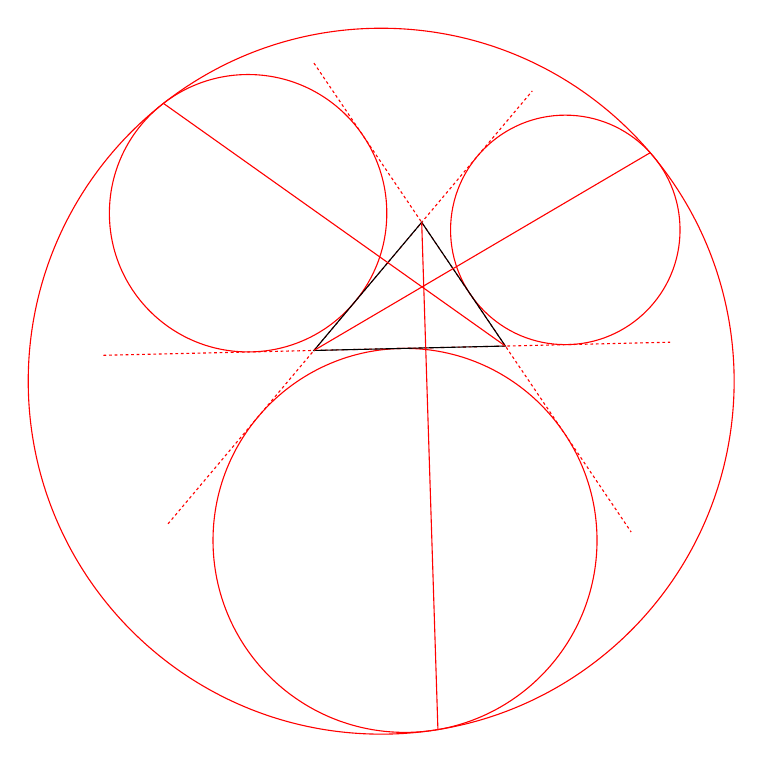
\begin{tikzpicture}[x=1pt,y=1pt]
\draw[red, dash pattern=on 1pt] (39.58,-139.33) -- (244.30,-134.61);
\draw[red, dash pattern=on 1pt] (62.92,-200.22) -- (194.53,-43.80);
\draw[red, dash pattern=on 1pt] (115.64,-33.74) -- (230.26,-203.19);
\draw[red] (206.46,-94.01) circle (41.46);
\draw[red] (91.84,-87.99) circle (50.12);
\draw[red] (148.54,-206.21) circle (69.38);
\draw[red] (139.93,-148.68) circle (127.54);
\draw (184.80,-135.98) -- (154.57,-91.28) -- (115.63,-137.58) -- cycle;
\draw[red] (154.57,-91.28) -- (160.43,-274.56);
\draw[red] (115.63,-137.58) -- (237.14,-66.12);
\draw[red] (184.80,-135.98) -- (61.26,-48.30);
\end{tikzpicture}
\end{document}
